\section{背景减 - Background Substraction}

\begin{frame}
    \frametitle{背景减技术简介}

    \begin{enumerate}
        \item 背景减(Background Substraction)是一种被广泛使用的动态目标检测技术。背景减技术通常需要从静止的相机中提取出``前景''
        \item 为了计算前景蒙版,在当前帧和背景之间进行减法运算,减去前几帧中习得的``背景''
    \end{enumerate}

    \begin{figure}
        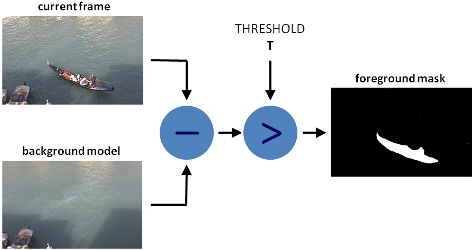
\includegraphics[width=0.618\textwidth]{images/Background_Subtraction_Tutorial_Scheme.png}
        \caption{背景减技术示意}
    \end{figure}

\end{frame}


\begin{frame}
    \frametitle{利用OpenCV实现背景减}

    OpenCV提供了类cv::BackgroundSubstractor作背景减。在本次实验中,我们小组尝试了MOGS和KNN两种实现方法,并作对比
\end{frame}